\documentclass[a4paper]{article}
\usepackage{amsmath}  % Paket notwendig für \dfrac
\usepackage[utf8]{inputenc}
\usepackage[german]{babel}
\usepackage{graphicx}
\usepackage{array}
\usepackage{fancyhdr}
\usepackage{lastpage} % Paket zur Bestimmung der Gesamtseitenzahl
\usepackage{geometry} % Paket zur Anpassung der Ränder
\usepackage[datesep=/,style=ddmmyyyy]{datetime2} % Paket zur Formatierung des Datums
\usepackage{setspace} % Enthält das setspace-Paket
\usepackage{enumitem}
\usepackage{amssymb} % Für zusätzliche Symbole
\usepackage{indentfirst}
\usepackage{hyperref}
\usepackage{array}
\usepackage{booktabs}

\usepackage{titlesec} % Enthält das titlesec-Paket
% Formatierung des Abschnittstitels mit kleinerer Schriftgröße
\titleformat{\section}
{\normalfont\large\bfseries}{\thesection}{1em}{}

% Festlegung der Seiten- und Kopfzeilenränder
\geometry{
	left=20mm,
	right=20mm,
	top=40mm,
	bottom=30mm,
	headsep=20mm
}

\pagestyle{fancy}
\fancyhf{} % Standardkopf- und Fußzeilen leeren
\renewcommand{\headrulewidth}{0pt} % Entfernt die Linie in der Kopfzeile
\renewcommand{\footrulewidth}{0.4pt} % Linie oberhalb der Fußzeile

\fancyhead[C]{ % Zentrierter Inhalt in der Kopfzeile
	\begin{tabular}{|m{3.5cm}|m{9.0cm}|m{3.5cm}|}
		\hline
		\begin{minipage}[c][2.0cm][c]{3.5cm}
			\centering
			
\includegraphics[width=2.98cm,height=1.25cm]{logo.png}
		\end{minipage} &
		\begin{minipage}[c][2.0cm][c]{9cm}
			\centering
			\hyphenpenalty=10000 % Vermeidet Trennungen
			\vspace*{\fill} % Flexibler vertikaler Abstand vor dem Text
			\begin{spacing}{1.5} % Erhöht den Zeilenabstand auf 1,25
				{\large \textbf{Induktor zur Reduzierung von transitorischem \textit{Inrush}-Strom in Kondensatoren}}
			\end{spacing}
			\vspace*{\fill} % Flexibler vertikaler Abstand nach dem Text
		\end{minipage} &
		\begin{minipage}[c][2.0cm][c]{3.5cm}
			\raggedleft
			Ausgabe: \DTMtoday \\
			Seite: \thepage/\pageref{LastPage}
		\end{minipage} \\
		\hline
	\end{tabular}
}

% Inhalt der Fußzeile
\fancyfoot[L]{%
	\begin{tabular}[b]{@{}l@{}}
		\href{http://www.dax.energy}{www.dax.energy}
	\end{tabular}
}
\fancyfoot[C]{%
	\begin{tabular}[b]{@{}c@{}}
		\href{mailto:comercial@dax.energy}{comercial@dax.energy}
	\end{tabular}
}
\fancyfoot[R]{%
	\begin{tabular}[b]{@{}r@{}}
		+55 41 99940-3744 \\ 3626-2072
	\end{tabular}
}

\begin{document}
\setstretch{1.25} % Definiert den Zeilenabstand auf 1,25

\section{Kontext}
Das Einschalten eines Kondensatorbänks (Abbildung \ref{fig:picture1}) durch das Schließen eines Leistungsschalters führt zu einem hohen transitorischen Spitzenstrom (Abbildung \ref{fig:picture2}), der als Inrush bezeichnet wird. Die Größe und Frequenz dieses transitorischen Spitzenstroms hängen ab von:
\begin{itemize}[label=\textendash]
\item der angelegten Spannung (Punkt auf der Spannungswelle beim Schließen);
\item der äquivalenten Kapazität des Stromkreises;
\item der Induktivität im Stromkreis (Menge und Ort);
\item der Ladung auf dem Kondensatorbank zum Zeitpunkt des Schließens;
\item jeder Dämpfung des Stromkreises aufgrund von Schließwiderständen oder anderen Widerständen im Stromkreis.
\end{itemize}

\section{Eingabedaten des Kondensatorbänks}
\begin{itemize}[label=\textendash]
	\item Blindleistung  = {{potencia_reativa_do_banco}}
	\item Dreiphasenspannung  = {{tensao_trifasica}}
	\item Einphasenspannung  = {{tensao_monofasica}}
	\item Kurzschlussstrom  = {{corrente_de_curto}}
\end{itemize}

\begin{center}
	% INSERT_TABLE_HERE
\end{center}

\section{Erste Überlegungen}

Der transitorische \textit{Inrush}-Strom ist kein limitierender Faktor bei isolierten Kondensatorbankanwendungen. Wenn jedoch Kondensatorbänke \textit{Back-to-Back} geschaltet werden, d. h. wenn ein Bank eingeschaltet wird, während ein anderer Bank an denselben Sammelschiene angeschlossen ist, fließen Hochfrequenzströme mit hoher Amplitude zwischen dem eingeschalteten Bank und den bereits eingeschalteten Bänken.

\begin{figure}[!hbp]
	\centering
	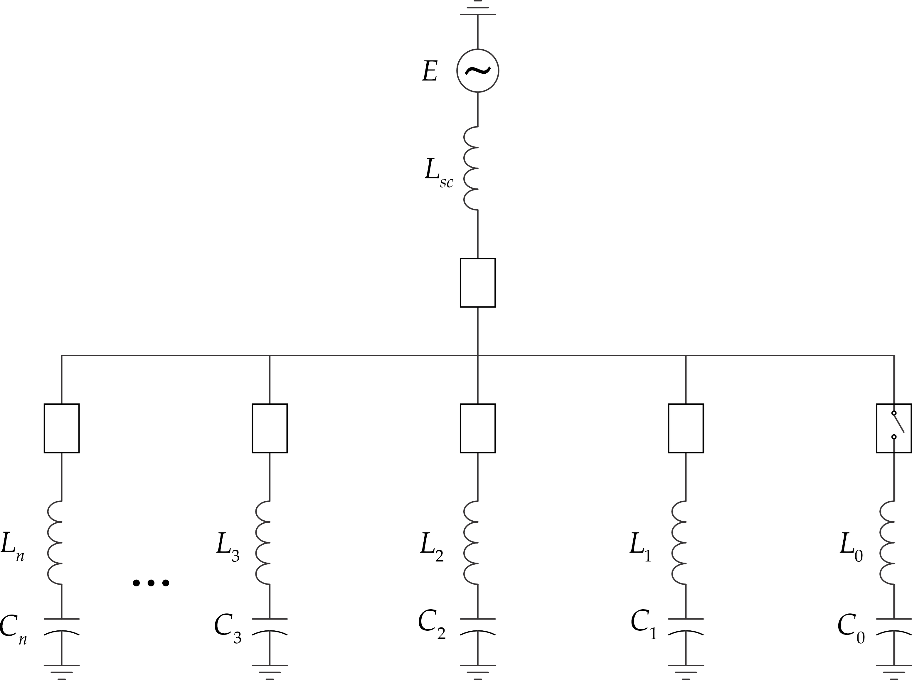
\includegraphics{Picture1.png}
	\caption{Kondensatorbanksystem.}
	\label{fig:picture1}
\end{figure}

Dieser oszillierende Strom ist nur durch den Widerstand des Kondensatorbanks und den Stromkreis zwischen den energisierten Bänken und dem geschalteten Bank (Bank \#0) begrenzt, der in der Regel innerhalb eines Bruchteils eines Systemfrequenzzyklus auf Null abklingt. Im Falle des \textit{Back-to-Back}-Schaltens ist die vom Generator gelieferte Komponente bei einer niedrigeren Frequenz (60 Hz) und so klein im Vergleich zum \textit{Inrush}-Strom, dass sie vernachlässigt werden kann \href{https://ieeexplore.ieee.org/document/7035261}{[ANSI/IEEE C37.012-1979]}.

\section{Ergebnisse}
\begin{figure}[!hbp]
	\centering
	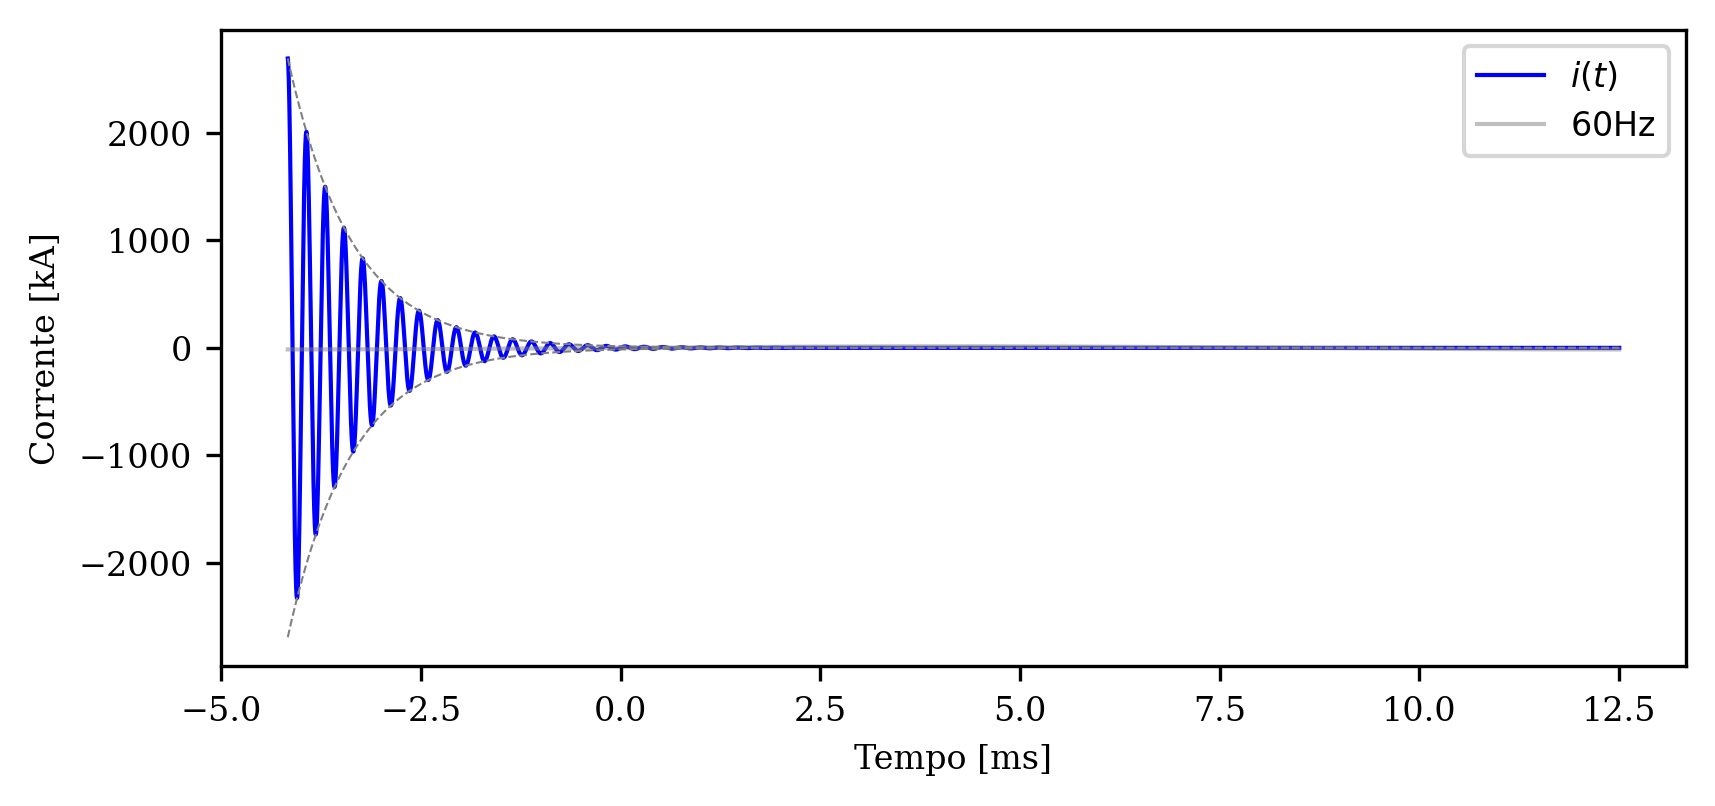
\includegraphics{Correntes.png}
	\caption{Momentanstrom in der eingeschalteten Kondensatorbank in einem Zyklus der Grundfrequenz.}
	\label{fig:picture2}
\end{figure}

Die mit dem gewählten Reaktor ($L_{reator} = {{indutancia_escolhida}} \, \mu \rm{H} $) erhaltenen Werte sind:
\begin{itemize}[label=\textendash]
	\item Spitzenstrom: {{corrente_pico}};
	\item Schwingungsfrequenz: {{frequencia_oscilacao}}Hz;
	\item Inrush-Strom / Nennstrom: {{inrush_inominal}}
\end{itemize}

\section{Fazit}
{{conclusao1}}

\section{Referenzen}

\noindent
\begin{tabular}{p{0.2cm} p{15.8cm}}
    \href{https://ieeexplore.ieee.org/document/7035261}{[1]} &
    \begin{minipage}[t]{15.8cm}
        IEEE Application Guide for Capacitance Current Switching for AC High-Voltage Circuit Breakers Rated on a Symmetrical Current Basis, in ANSI/IEEE C37.012-1979, vol., no., pp.1-54, 6 Feb. 1979, doi: 10.1109/IEEESTD.1979.7035261.
    \end{minipage} \\

    \href{https://ieeexplore.ieee.org/document/9574631}{[2]} &
    \begin{minipage}[t]{15.8cm}
        IEEE Approved Draft Standard Requirements for Capacitor Switches for AC Systems (1 kV to 38 kV), in IEEE PC37.66/D10, October 2021, vol., no., pp.1-35, 13 Dec. 2021.
    \end{minipage} \\


    \href{https://webstore.iec.ch/publication/62785}{[3]} &
    \begin{minipage}[t]{15.8cm}
       IEC 62271-100 High-voltage switchgear and controlgear - Part 100: Alternating-current circuit-breakers
    \end{minipage} \\

    \href{https://ieeexplore.ieee.org/document/5318709}{[4]} &
    \begin{minipage}[t]{15.8cm}
        IEEE Standard for AC High-Voltage Circuit Breakers Rated on a Symmetrical Current Basis--Preferred Ratings and Related Required Capabilities for Voltages Above 1000 V, in IEEE Std C37.06-2009, vol., no., pp.1-56, 6 Nov. 2009, doi: 10.1109/IEEESTD.2009.5318709.
    \end{minipage} \\

    \href{https://cdn.standards.iteh.ai/samples/101972/4e7e06bd66d2443da668b8e0c6c60512/IEC-62271-100-2021.pdf}{[5]} &
    \begin{minipage}[t]{15.8cm}
        IEC 62271-100 High-voltage switchgear and controlgear – Part 100: Alternating-current circuit-breakers.
    \end{minipage} \\

    \href{https://www.normas.com.br/autorizar/visualizacao-nbr/313/identificar/visitante}{[6]} &
    \begin{minipage}[t]{15.8cm}
        NBR 5282 Parallelleistungskondensatoren für nominale Spannungsanlagen über 1000 V.
    \end{minipage} \\
\end{tabular}

% Platz für Unterschriften
\noindent % Verhindert Einrückung
\begin{minipage}[t]{0.5\textwidth} % Beginnt die erste Spalte für die Unterschrift
	\centering % Zentriert den Text
	\vspace{5cm} % Platz reserviert für die Unterschrift
	\rule{6cm}{0.4pt}\\ % Linie für Unterschrift
	\textbf{Angelo A. Hafner}\\ % Name
	Elektroingenieur\\ % Titel
	CONFEA: 2.500.821.919\\ % Registrierungsnummer
	CREA/SC: 045.776-5\\ % Eine andere Registrierungsnummer
	aah@dax.energy % E-Mail
\end{minipage}%
\hfill % Abstand zwischen den Spalten
\begin{minipage}[t]{0.5\textwidth} % Beginnt die zweite Spalte für die Unterschrift
	\centering % Zentriert den Text
	\vspace{5cm} % Platz reserviert für die Unterschrift
	\rule{6cm}{0.4pt}\\ % Linie für Unterschrift
	\textbf{Tiago Machado}\\ % Name
	Geschäftsführer\\ % Titel
	Mobile: +55 41 99940-3744\\ % Kontakt
	tm@dax.energy % E-Mail
\end{minipage}

\end{document}
